\documentclass{bioinfo}
\copyrightyear{2005}
\pubyear{2005}

\begin{document}
\firstpage{1}

\title[bwa-meth]{Fast and accurate alignment of long bisulfite-seq reads}
\author[Pedersen \textit{et~al}]{
Brent S. Pedersen\,$^{1,}
\footnote{To whom correspondence should be addressed.  Email: bpederse@gmail.com}$,
Kenneth Eyring\,$^{1}$,
Subhajyoti De\,${1,2}$,
Ivana V. Yang\,$^{1}$
and David A. Schwartz\,$^1$%
}
\address{
    $^{1}$Department of Medicine, University of Colorado Denver, School of Medicine, Denver, Colorado, USA. 80045 \\
    $^{2}$University of Colorado Cancer Center, Molecular Oncology Program,
    Aurora, Colorado, United States
}

\history{Received on XXXXX; revised on XXXXX; accepted on XXXXX}

\editor{Associate Editor: XXXXXXX}

\maketitle

\begin{abstract}

    %http://www.oxfordjournals.org/our_journals/bioinformatics/for_authors/general.html

\section{Summary:}
Longer sequencing reads, with at least 200 bases per template are now common.
While traditional aligners have adopted new strategies to improve the mapping of longer reads,
aligners specific to bisulfite-sequencing were optimized when much shorter reads
were the norm. We sought to perform the first comparison using longer reads to
determine which aligners were most accurate and efficient and to evaluate a novel
software tool, \textit{bwa-meth}, built on a traditional mapper that supports
insertions, deletions and clipped alignments. We gauge accuracy by comparing
the number of on and off-target reads from a targeted sequencing project
and by simulations.

\section{Availability and Implementation:}
The benchmarking scripts and the \textit{bwa-meth} software are available at
https://github/com/brentp/bwa-meth/ under the MIT License.

\section{Contact:} \href{bpederse@gmail.com}{bpederse@gmail.com}
\section{Supplementary information:} 
Supplemental Information I
\end{abstract}

\section{Introduction}
Bisulfite sequencing (BS-Seq) is a common way to explore methylation status.
As a result, software \citep{frithlast,methylcoder,gsnap,krueger2011,bsmap}
have been developed to map sequence reads treated with bisulfite to a reference genome.
Many of these were developed on and optimized for shorter reads
than what are common from today's sequencers. Many of these have compared alignment
statistics on real \citep{methylcoder,bsmap} and simulated \citep{frithlast} reads,
however these are limited by knowledge of the ground-truth and assumptions of
the simulation, respectively.

Here, we present an analysis of current BS-Seq mappers including the "four-base" aligners
Last \citep{frithlast}, GSNAP \citep{gsnap} and BSMAP \citep{bsmap} and the most-used
"three-base" aligner Bismark \citep{krueger2011} which performs \emph{in silico} conversion
of cytosines to thymines. In addtion, we introduce our
own, simple three-base aligner that wraps \textit{BWA mem} \citep{bwamem}.

The comparison is performed on 100-base paired-end reads
which are of modest length by current standards, but, to our knowledge, longer than
utilized in any comparison. We hypothesized that having long, paired reads, with up
to 200 bases from the same genomic region, could change the decision on which
alignment method performed the best. 
We found limitations to exisiting aligners including the writing of large temporary
files, high memory-use, long run-time, output that was not suitable for consumption by
traditional tools, or some combination of these inconveniences. We wrote
a BS-Seq aligner based on BWA mem \citep{bwamem} to address these
limitations. This new aligner, 
\textit{bwa-meth}, allows indels, clipped alignments, and it never writes a
temporary-file of the reads to disk, instead streaming the \emph{in silico} converted
reads directly to the aligner.

\section{Approach}
We introduce a novel approach for determining the accuracy of an aligner;
we utilize a dataset from Agilent's SureSelect Mouse Methyl-Seq kit which
captures about
99 million bases from high CpG-density regions in the mouse genome (a similar
approach is available for human regions).
We gauge an aligner by the number of reads in the capture area as compared
to outside of the capture area. While there will be off-target capture, all
aligners are subject to the same assumptions. With those constraints, we can
plot a receiver operating curve (ROC) with true positives as reads within
and false positives as reads outside of the target regions.
This will be the first comparison of BS-Seq aligners on real data where accuracy
can be assessed in an unbiased manner.

In addition, we perform simulations with 100-base paired-end reads using
the software from the authors of Bismark. All data were aligned to mouse
genome version \textit{mm10}.


\begin{methods}
\section{Methods}
We aligned real and simulated data, both trimmed by quality and
un-trimmed, using the software and versions in Table \ref{Tab:01}.
We evaluated a few parameters for each method and report only the
best-performing here. We trimmed the data based on quality
using Sickle (https://github.com/najoshi/sickle) default parameters.
We considered a real read to be in the target region if it
was within 101 bases of the target area. 

\begin{table}[!t]
\processtable{Alignment Methods Compared\label{Tab:01}}
{\begin{tabular}{lll}\toprule
software & version & command\\\midrule
bismark & 0.10.1 & bismark --gzip --maxins 1000 -n 3 -l 20 --bam\\
bsmap & 2.74 & bsmap -s12 -v3 -m0 -x1000 -S42 -n0 -s12 -I1\\
bwa-meth & 0.06 & bwa-meth\\
gsnap & 2013-03-21 & gsnap -B4 --npaths 1 --quiet-if-excessive\\
last & 392 & last-bisulfite-paired.sh\\\botrule
\end{tabular}}{We used a modified version of the calling script for last}
\end{table}

\end{methods}

\begin{figure}[!tpb]%figure1
    \centerline{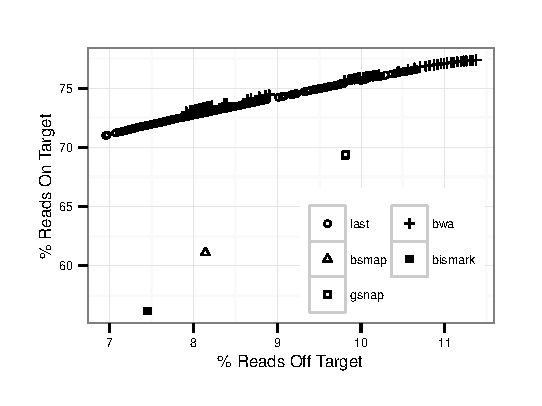
\includegraphics[width=86mm]{qual-plot-real}}
    \caption{Percent of paired-end, 100-base reads on (y) and off (x) target for the tested aligners. Aligners that report mapping quality are shown as connected dots for each quality cut-off. Reads are limited to those considered as primary, mapped alignments by the aligner.}\label{fig:01}
\end{figure}

\section{Discussion}

While \textit{bwa-meth} can align single-end reads, it has been optimized for
paired-end reads from the directional protocol, we show its utility here on real
and simulated data. Since it consists
of fewer than 400 lines of code (compared to, e.g. about 8000 for Bismark) and runs
quickly, it can be used as a platform to test other optimizations.

\subsection{Accuracy}
Of the aligners tested, only two report a range of mapping quality
scores--an indicator of the aligner's confidence in the alignment. For
those, we vary the score from 1 to the maximum, 255, to draw an ROC-like
curve showing the trade-off between sensitivity and specificity. For the
other aligners, we plot their single location. Figure \ref{fig:01} shows
the on and off-target reads for our real paired-end data. Last and 
\textit{bwa-meth} align the most reads on target with a low percent
of off-target reads, but Last provides better control over the number
of off-target reads. Bismark also has a low percentage of off-target reads.

Similar comparisons are shown in  Supplemental Figures 2
for trimmed data and for simulated data in Supplemental Figures 3 and 4.
\textit{Bwa-meth} does out-perform Last (along with the other aligners)
for simulated data although GSNAP also performs very well.

\subsection{Computational Resources}
Within reason, we are more interested in the accuracy of a
method than the speed. In general, the order of aligners from fastest to
slowest is: Last, \textit{bwa-meth}, Bismark, GSNAP, bsmap. However, Bismark
is the fastest by a factor of 2 on the simulated data. We report the exact 
timings and maximum memory use in Supplemental Information.
Bsmap uses the least disk, never writing an index of the reference genome
and only writing the alignment files. All other aligners write an index of
the reference genome. Last and bismark both write additional copies of the
reads to disk. This is to aid in parallelization in the case of Last and to
write the \emph{in silico} converted reads in the case of bismark. While
these could presumably be addressed in either case, they are considerations
at the time of writing. It is common to get 10GB of compressed sequence data
from 10 samples. If an aligner must write copies of the
sequence data, this increases the storage requirements enough to be a
consideration in our experience. \textit{Bwa-meth} avoids writing the \emph{in silico}
converted reads to disk by streaming them directly to the aligner.
None of the programs used an inordinate amount of memory, however, due to
the parallelization strategy, Last did require about 10GB of shared memory
per process.


%%%%%%%%%%%%%%%%%%%%%%%%%%%%%%%%%%%%%%%%%%%%%%%%%%%%%%%%%%%%%%%%%%%%%%%%%%%%%%%%%%%%%
%
%     please remove the " % " symbol from \centerline{\includegraphics{fig01.eps}}
%     as it may ignore the figures.
%
%%%%%%%%%%%%%%%%%%%%%%%%%%%%%%%%%%%%%%%%%%%%%%%%%%%%%%%%%%%%%%%%%%%%%%%%%%%%%%%%%%%%%%






\section{Conclusion}
We have shown that BS-Seq aligners built for and optimized with shorter reads
with end-to-end alignments can be out-performed by sending \emph{in silico}
converted reads to a modern aligner such as \textit{BWA mem} \citep{bwamem}.
We have utilized a new technology that captures CpG-rich regions to compare
accuracy and speed of \textit{bwa-meth} to existing aligners.
It demonstrates greater accuracy than other aligners and outputs quality
scores which can be used to filter which aligments are considered in
downstream analysis.

\section*{Acknowledgement}

\paragraph{Funding\textcolon} This was funded by R01 HL097163, R01 HL101251, 1I01BX001534, RC2 HL101715, N01 AI90052, and S10 RR031832.

%\bibliographystyle{natbib}
%\bibliographystyle{achemnat}
%\bibliographystyle{plainnat}
%\bibliographystyle{abbrv}
%\bibliographystyle{bioinformatics}
%
%\bibliographystyle{plain}
%
%\bibliography{Document}


%\begin{thebibliography}{}
\bibliographystyle{natbib}
    \bibliography{document}
%\end{thebibliography}
\end{document}
